\documentclass[
  bibliography=totoc,     % Literatur im Inhaltsverzeichnis
  captions=tableheading,  % Tabellenüberschriften
  titlepage=firstiscover, % Titelseite ist Deckblatt
]{scrartcl}

% Paket float verbessern
\usepackage{scrhack}

% Warnung, falls nochmal kompiliert werden muss
\usepackage[aux]{rerunfilecheck}

% unverzichtbare Mathe-Befehle
\usepackage{amsmath}
% viele Mathe-Symbole
\usepackage{amssymb}
% Erweiterungen für amsmath
\usepackage{mathtools}

% Fonteinstellungen
\usepackage{fontspec}
% Latin Modern Fonts werden automatisch geladen
% Alternativ zum Beispiel:
%\setromanfont{Libertinus Serif}
%\setsansfont{Libertinus Sans}
%\setmonofont{Libertinus Mono}

% Wenn man andere Schriftarten gesetzt hat,
% sollte man das Seiten-Layout neu berechnen lassen
\recalctypearea{}

% deutsche Spracheinstellungen
\usepackage[ngerman]{babel}


\usepackage[
  math-style=ISO,    % ┐
  bold-style=ISO,    % │
  sans-style=italic, % │ ISO-Standard folgen
  nabla=upright,     % │
  partial=upright,   % │
  mathrm=sym,        % ┘
  warnings-off={           % ┐
    mathtools-colon,       % │ unnötige Warnungen ausschalten
    mathtools-overbracket, % │
  },                       % ┘
]{unicode-math}

% traditionelle Fonts für Mathematik
\setmathfont{Latin Modern Math}
% Alternativ zum Beispiel:
%\setmathfont{Libertinus Math}

\setmathfont{XITS Math}[range={scr, bfscr}]
\setmathfont{XITS Math}[range={cal, bfcal}, StylisticSet=1]

% Zahlen und Einheiten
\usepackage[
  locale=DE,                   % deutsche Einstellungen
  separate-uncertainty=true,   % immer Unsicherheit mit \pm
  per-mode=symbol-or-fraction, % / in inline math, fraction in display math
]{siunitx}

% chemische Formeln
\usepackage[
  version=4,
  math-greek=default, % ┐ mit unicode-math zusammenarbeiten
  text-greek=default, % ┘
]{mhchem}

% richtige Anführungszeichen
\usepackage[autostyle]{csquotes}

% schöne Brüche im Text
\usepackage{xfrac}

% Standardplatzierung für Floats einstellen
\usepackage{float}
\floatplacement{figure}{htbp}
\floatplacement{table}{htbp}

% Floats innerhalb einer Section halten
\usepackage[
  section, % Floats innerhalb der Section halten
  below,   % unterhalb der Section aber auf der selben Seite ist ok
]{placeins}

% Seite drehen für breite Tabellen: landscape Umgebung
\usepackage{pdflscape}

% Captions schöner machen.
\usepackage[
  labelfont=bf,        % Tabelle x: Abbildung y: ist jetzt fett
  font=small,          % Schrift etwas kleiner als Dokument
  width=0.9\textwidth, % maximale Breite einer Caption schmaler
]{caption}
% subfigure, subtable, subref
\usepackage{subcaption}

% Grafiken können eingebunden werden
\usepackage{graphicx}

% schöne Tabellen
\usepackage{tabularray}
\UseTblrLibrary{booktabs, siunitx}

% Verbesserungen am Schriftbild
\usepackage{microtype}

% Literaturverzeichnis
\usepackage[
  backend=biber,
]{biblatex}
% Quellendatenbank
\addbibresource{lit.bib}
\addbibresource{programme.bib}

% Hyperlinks im Dokument
\usepackage[
  german,
  unicode,        % Unicode in PDF-Attributen erlauben
  pdfusetitle,    % Titel, Autoren und Datum als PDF-Attribute
  pdfcreator={},  % ┐ PDF-Attribute säubern
  pdfproducer={}, % ┘
]{hyperref}
% erweiterte Bookmarks im PDF
\usepackage{bookmark}

% Trennung von Wörtern mit Strichen
\usepackage[shortcuts]{extdash}

\author{%
  Vincent Wirsdörfer\\%
  \href{mailto:vincent.wirsdoerfer@udo.edu}{authorA@udo.edu}%
  \and%
  Joris Daus\\%
  \href{mailto:joris.daus@udo.edu}{authorB@udo.edu}%
}
\publishers{TU Dortmund – Fakultät Physik}


\begin{document}
\section{Zielsetzung}

In dem folgend protokollierten Versuch werden gedämpfte und erzwungene Schwingungen am Beispiel des \emph{RCL-}Kreises
untersucht. Das konkrete Ziel besteht darin, die zeitliche Abhängigkeit der Amplitude einer gedämpften Schwingung zu
analysieren, um den Dämpfungswiderstand zu ermitteln. Ferner wird die Frequenzabhängigkeit der Kondensatorspannung an einem
Serienresonanzkreis gemessen.

\section{Theorie}
\label{sec:Theorie}

Die elementaren Bestandteile eines ungedämpften \emph{LC-}Kreises sind ein Kondensator mit Kapazität $C$ und eine 
Spule mit Induktivität $L$. Im idealen Fall repräsentiert dieser Schaltkreis einen ständigen Energieaustausch durch 
sich abwechselnd aufbauende elektrische und magnetische Felder. Zu Beginn der Systembetrachtung wird durch einen 
geladenen Kondensator ein E-Feld erzeugt. Die Ladung am Kondensator strebt jedoch eine Minimierung der vorliegenden 
Potentialdifferenz an, weswegen die Ladungsträger durch den Schaltkreis fließen und dabei die Spule durchlaufen. 
Dementsprechend wird in der Spule ein B-Feld erzeugt, wodurch das immer kleiner werdende E-Feld kompensiert wird. Nach
einer gewissen Zeit wird jedoch auch das B-Feld allmählich schwächer, da der Stromfluss geringer wird, wohingegen die 
Ladungsmengen am Kondensator erneut steigen. Nach der \emph{Lenz'schen Regel}\footnote{Die Lenz'sche Regel besagt, dass der
Induktionsstrom immer seiner Ursache entgegengesetzt ist.} entsteht somit ein dem Anfangszustand entgegengesetztes E-Feld.
Im späteren Verlauf wird durch den daraus folgenden Stromfluss wieder ein B-Feld erzeugt, was wiederum in einem E-Feld 
mündet. Dieser Vorgang wiederholt sich periodisch.\\
Nun wird in dem Schaltkreis ein ohm'scher Widerstand $R$ implementiert. Eine mögliche Realisierung dessen ist in Abbildung 
\ref{fig:RCL-Kreis} zu sehen.

\begin{figure}
    \centering
    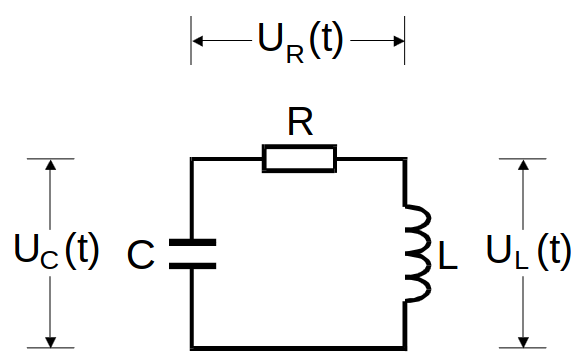
\includegraphics[height=5cm]{RCL_Kreis.png}
    \caption{Aufbau eines \emph{RCL-}Kreises \cite{Versuchsanleitung_v354}.}
    \label{fig:RCL-Kreis}
\end{figure}

\noindent Hierbei wirkt der Widerstand $R$ als Dämpfung des Schwingkreises. Die vorher transportierte elektrische Energie wird nun 
über die Zeit auch in Wärmeenergie umgewandelt, weswegen, von einer graphischen Perspektive betrachtet, die Elongation der 
Schwingungen mit der Zeit geringer werden.\\
Um nun genaue mathematische Aussagen über das Verhalten des gedämpften Schwingkreises treffen zu können, wird mittels des 
\emph{2. Kirchhoff'schen Gesetzes}\footnote{Das 2. Kirchhoff'sche Gesetz postuliert, dass die Summe aller Spannungsabfälle
in einer Masche (geschlossener Stromkreis), Null ergibt.} eine Differentialgleichung aufgestellt. Diese nimmt 
allgemein die folgende Gestalt an:

\begin{equation}
\label{eqn:Kirchhoff2}
    U_\text{L}(t) + U_\text{R}(t) + U_\text{C}(t) = 0
\end{equation}

\noindent All diese Spannungen lassen sich ebenfalls über die Stromstärke $I$ ausdrücken:

\begin{align*}
    U_\text{L}(t) &= L\dot{I}(t) \\
    U_\text{R}(t) &= RI(t) \\
    U_\text{C}(t) &= \frac{Q(t)}{C} \\
\end{align*}

\noindent Durch Einsetzen dieser Ausdrücke in \eqref{eqn:Kirchhoff2} sowie einfaches zeitliches Differenzieren ergibt sich

\begin{equation*}
    \ddot{I}(t) + \frac{R}{L}\dot{I}(t) + \frac{1}{LC}I(t) = 0
\end{equation*}

\noindent als die auszuwertende homogene Differentialgleichung zweiter Ordnung. Diese hat mittels eines geeigneten Exponentialansatzes 
folgende Lösung:

\begin{equation}
\label{eqn:solutionDGL}
    I(t) = e^{-2\pi\mu{}t}\left(A_1e^{i2\pi\nu{}t} + A_2e^{-i2\pi\nu{}t}\right)
\end{equation}

\noindent Hierbei sind die Konstanten $A_1$ und $A_2$ zwei komplexe Zahlen. Die Größen $\mu$ und $\nu$ stehen 
für folgende Ausdrücke:

\begin{gather*}
    \mu \coloneqq \frac{R}{4\pi{}L} 
    \label{eqn:mu}\\
    \nu \coloneqq \frac{1}{2\pi}\sqrt{\frac{1}{LC} - \frac{R²}{4L²}}
\end{gather*}
\section{Vorbereitung}

Das Abklingverhalten der Schwingung lässt sich nun in verschiedene Fälle unterscheiden. Zum einen kann der Ausdruck 
unter der Wurzel reell sein. Dies ist genau dann der Fall, wenn die Abschätzung

\begin{equation}
\label{eqn:reell}
    \frac{1}{LC} > \frac{R²}{4L²}
\end{equation}

\noindent gilt. Die allgemeine Lösung der Differentialgleichung aus \eqref{eqn:solutionDGL} lässt sich in diesem Fall 
schreiben als

\begin{equation*}
    I(t) = A_0e^{-2\pi\mu{}t}\cos\left(2\pi\nu{}t + \varphi\right).
\end{equation*}

\noindent Daran lässt sich erkennen, dass die gedämpfte Schwingung für $t \rightarrow \infty$ gegen null strebt, wobei
die Abklingdauer $T_\text{ex}$ definiert ist durch:

\begin{equation}
    T_\text{ex} \coloneqq \frac{1}{2\pi\mu}
    \label{eqn:abklingdauer}
\end{equation}

\noindent Für den Fall, dass $\nu$ imaginär ist, muss der Radikand negativ sein. Es gilt also die inverse Abschätzung 

\begin{equation}
\label{eqn:imaginaer}
    \frac{1}{LC} < \frac{R²}{4L²}.
\end{equation}

\noindent Mit Bezug auf \eqref{eqn:solutionDGL} lässt sich somit 

\begin{equation*}
    I(t) \propto e^{\left(-2\pi\mu + i2\pi\nu\right)t}
\end{equation*}

\noindent als ebenfalls exponentiell abfallende Lösung klassifizieren.\\
Der in diesem Versuch wichtige Fall ist der sogenannte \textbf{aperiodische Grenzfall}. Dieser charakterisiert sich durch 
das Verschwinden der Größe $\nu$, was durch die Äquivalenz 

\begin{equation}
\label{eqn:Grenzfall}
    \frac{1}{LC} = \frac{R²}{4L²}
\end{equation}

\noindent erreicht werden kann. Die allgemeine Lösung \eqref{eqn:solutionDGL} vereinfacht sich nun auf 

\begin{equation*}
    I(t) = Ae^{-2\pi\mu{}t} = Ae^{-\frac{R}{2L}t},
\end{equation*}

\noindent wobei $A = A_1 + A_2$ ist. Bei diesem Fall verschwinden Dementsprechend die imaginären also oszillatorischen Anteile 
der Schwingung, weswegen beim aperiodischen Grenzfall das schnellste Abklingverhalten beobachtet werden kann.\\\\

\noindent Im zweiten Teil des Versuchs wird eine äußere Anregung in den Schaltkreis eingebaut. Daher wird auch von 
einer \textbf{erzwungenen Schwingung} gesprochen. Konkretisiert wird diese Anregung durch eine Wechselstromquelle mit 
der Kreisfrequenz $\omega$. Der modulierte Aufbau des $RCL$-Kreises wird in der folgenden Abbildung visualisiert.

\begin{figure}[H]
    \centering
    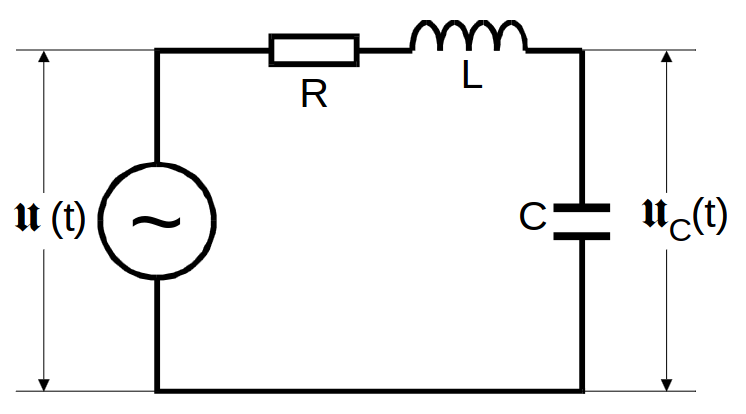
\includegraphics[height=4cm]{AnregungRCL.png}
    \caption{Aufbau eines angeregten $RCL$-Kreises \cite{Versuchsanleitung_v354}.}
    \label{fig:AnregungRCL}
\end{figure}

\noindent Mathematisch lässt sich diese Veränderung des Versuchsaufbaus durch einen zusätzlichen inhomogenen Teil in der 
ursprünglichen Differentialgleichung widerspiegeln:

\begin{equation*}
%\label{eqn:angeregteDGL}
    LC\ddot{U}_\text{C}(t) + RC\dot{U}_\text{C}(t) + U_\text{C}(t) = U_0e^{i\omega{}t}
\end{equation*}

\noindent Als Lösung dieser Differentialgleichung lässt sich berechnen:

\begin{equation*}
    U(t) = \frac{U_0\left(1 - LC\omega² - i\omega RC\right)}{\left(1 - LC\omega²\right)² + \omega²R²C²}
\end{equation*}

\noindent Ferner kann die Spannung auch in Abhängigkeit von der Frequenz angegeben werden:

\begin{equation*}
    U_\text{C}(t) = \frac{U_0}{\sqrt{\left(1 - LC\omega²\right)² + \omega²R²C²}}
\end{equation*}

\noindent An dieser Darstellung lässt sich herauskristallisieren, dass die Amplitude bei hohen Frequenzen 
$\left(\omega \rightarrow \infty\right)$ gegen null und bei kleinen Frequenzen $\left(\omega \rightarrow 0\right)$ 
gegen $U_0$ konvergiert. \\
Bei der sogenannten Resonanzfrequenz 

\begin{equation*}
    \omega_\text{res} = \sqrt{\frac{1}{LC} - \frac{R²}{2L²}}
\end{equation*}

\noindent kann die Kondensatorspannung einen größeren Maximalwert als die Amplitude der Erregerspannung erreichen.\\\\
Ein besonderer Fall der schwachen Dämpfung liegt genau dann vor, wenn die Äquivalenz  

\begin{equation*}
    \frac{R²}{2L²} << \frac{1}{LC}
\end{equation*}

\noindent erfüllt ist. In diesem Fall nähert sich die Resonanzfrequenz der Kreisfrequenz der ungedämpften Schwingung
$(\omega_\text{res} \approx \omega_0)$, wobei die Kreisfrequenz durch die \emph{Thomson'sche Schwingungsformel}\cite{Thomson}
gegeben ist als $\omega_0 = \sfrac{1}{\sqrt{LC}}$.\\
Wie bereits angesprochen, kann das Maximum der Kondensatorspannung die Amplitude der Erregerspannung bei Erreichen der 
Resonanzfrequenz übersteigen. Mathematisch präziser ausgedrückt kann $U_\text{C}$ um einen Faktor

\begin{equation}
    q = \frac{1}{\omega_{0}RC}
    \label{eqn:güte}
\end{equation}

\noindent größer werden als $U_0$. Dieser Faktor wird auch als \emph{Güte} des Schwingkreises tituliert. Im Kontext der Resonanzfrequenz ist 
ebenfalls die Breite der Resonanzkurve zu nennen. Unter der Voraussetzung einer schwachen Dämpfung $\left(\sfrac{R²}{2L²} << \sfrac{1}{LC}\right)$
kann die Breite der Resonanzkurve über die Näherung

\begin{equation*}
    \omega_\text{+} - \omega_\text{-} \approx \frac{R}{L}
\end{equation*}

\noindent beschrieben werden. $\omega_\text{+}$ und $\omega_\text{-}$ beschreiben dabei jene Frequenz, an denen $U_\text{C}$ auf den 
Bruchteil $\sfrac{1}{\sqrt{2}}$ des Maximalwertes abgefallen ist. Die Breite der Resonanzkurve kann als \enquote{Schärfe} der 
Resonanz betrachtet werden.


\section{Fehlerrechnung}
\label{sec:Fehlerrechnung}

Alle im Protokoll vermerkten Mittelwerte lassen sich über die folgende Formel berechnen:

\begin{equation}
\label{eqn:Mittelwert}
    \bar{x} = \frac{1}{N}\sum_{i=1}^N x_i
\end{equation}

Zudem lässt sich der dazugehörige Fehler des Mittelwerts wie folgt berechnen:

\begin{equation}
\label{eqn:Mittelwertfehler}
    \increment \bar{x} = \sqrt{\frac{1}{N\left(N-1\right)}\sum_{i=1}^N \left(x_i - \bar{x}\right)²}
\end{equation}

Entsteht ein neuer Fehler durch bereits fehlerbehaftete Größen, so wird die Gauß'sche Fehlerfortpflanzung angewendet:

\begin{equation}
\label{eqn:Fehlerfortpflanzung}
    \increment f = \sqrt{\sum_{i=1}^N \left(\frac{\partial f}{\partial x_i}\right)²\cdot\left(\increment x_i\right)²}
\end{equation}

\end{document}